\chapter{Hadoop e MapReduce}

\section{Introduzione al Framework Hadoop}
Il framework Hadoop, pur essendo stato proposto molti anni fa, introduce concetti di base che rimangono fondamentali nel mondo dell'elaborazione dei Big Data. I componenti principali di Hadoop includono un'infrastruttura di elaborazione distribuita, interamente basata sul paradigma di programmazione MapReduce, e il file system distribuito HDFS (Hadoop Distributed File System). Inoltre, all'ecosistema Hadoop sono associati molti altri progetti paralleli, come Spark e Hive (un database relazionale distribuito che sfrutta applicazioni MapReduce).

L'infrastruttura Hadoop è caratterizzata da alcune proprietà fondamentali:
\begin{itemize}
    \item \textbf{Astrazione ad alto livello (Separazione del \textit{What} dal \textit{How}):} Hadoop permette ai programmatori di concentrarsi esclusivamente su \textit{cosa} calcolare (implementando il paradigma MapReduce), mentre l'infrastruttura di Hadoop gestisce automaticamente il \textit{come}, occupandosi di tutte le complessità dei sistemi distribuiti, come lo scheduling dei task e la sincronizzazione.
    \item \textbf{Tolleranza ai guasti (Fault-tolerance):} I fallimenti dei singoli server (nodi) o dei task vengono gestiti automaticamente dal sistema Hadoop. Ad esempio, per evitare "single points of failure", vengono mantenute delle copie di backup (shadow copies/repliche) su server diversi che subentrano immediatamente nel caso in cui un nodo principale smetta di funzionare.
    \item \textbf{Alta disponibilità (High availability):} Il file system HDFS garantisce che lo storage distribuito sia sempre altamente disponibile e resiliente agli errori.
\end{itemize}

% FIGURA DA INSERIRE QUI
% Fonte: Slide "Hadoop: main components" 
% Descrizione: Schema ad albero che mostra l'infrastruttura fisica di Hadoop con Switch, Rack e Server (contenenti CPU, Memoria e Disco). Viene mostrato un esempio con un numero di repliche per chunk pari a 2.
\begin{figure}[H]
    \centering
    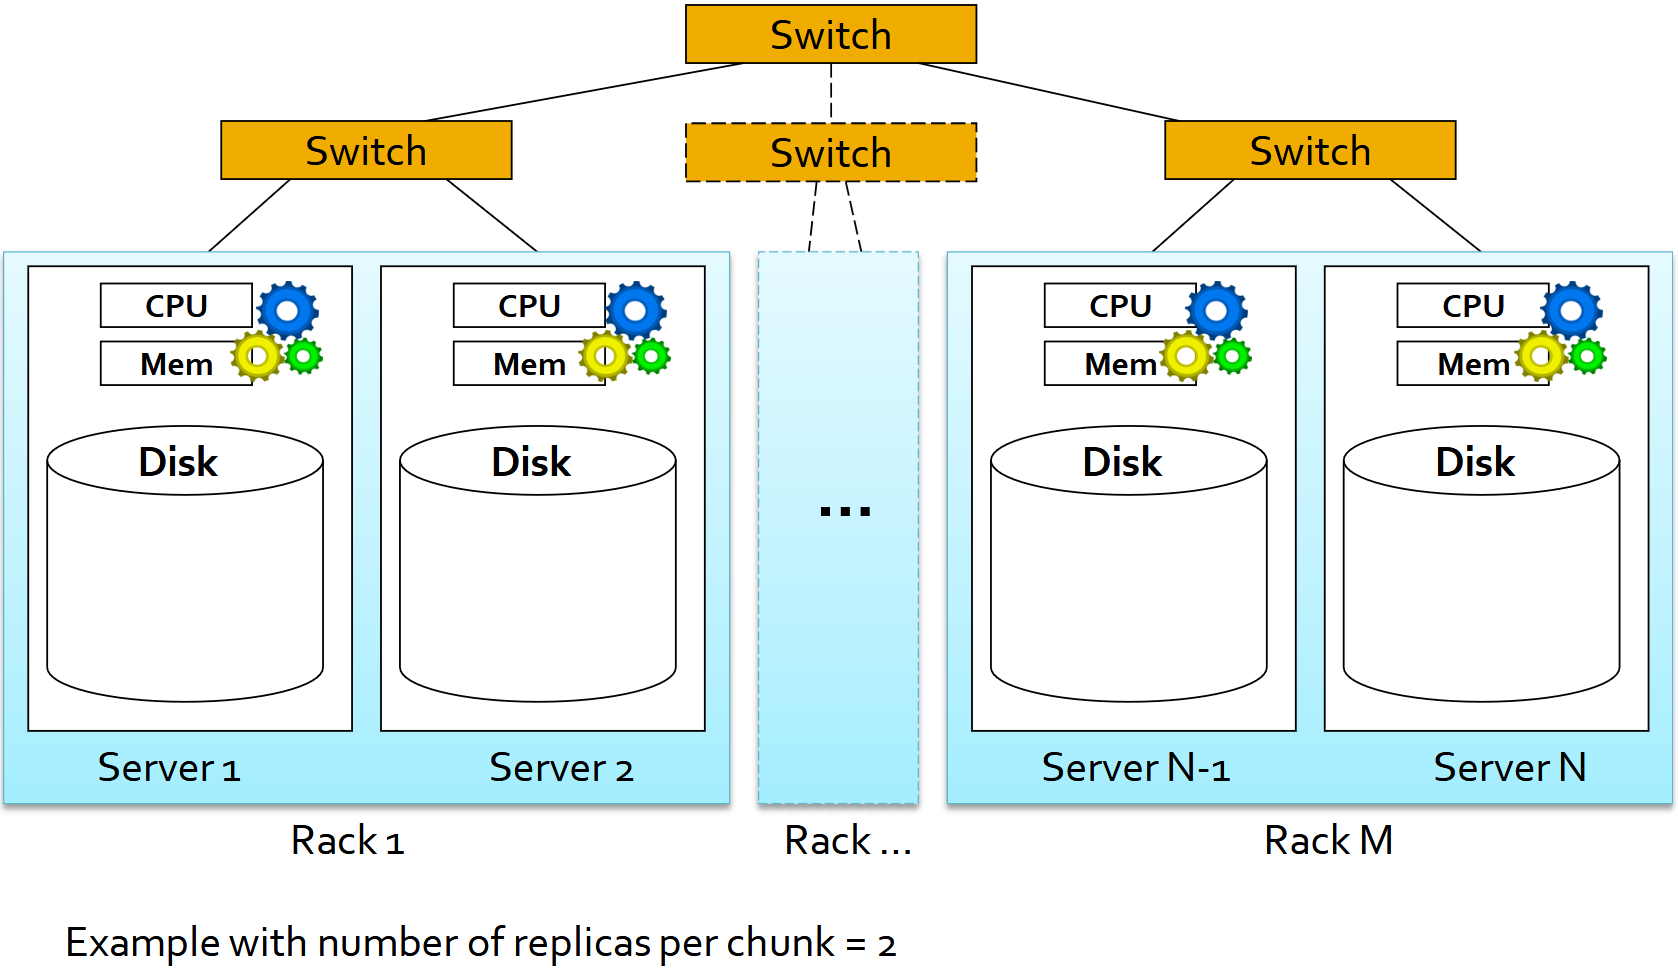
\includegraphics[width=0.8\textwidth]{capitoli/03_Intro_HadoopAndMapReduce/images/hadoop_infrastructure}
    \caption{Componenti fisici principali e gerarchia di rete in un cluster Hadoop.}
    \label{fig:hadoop_components}
\end{figure}

\section{Il Principio della Data Locality}
Nei sistemi distribuiti tradizionali (come gli ambienti HPC), l'approccio standard consiste nello spostare i dati verso i nodi di calcolo (server). Tuttavia, quando si ha a che fare con i Big Data, questo approccio non è scalabile per processare Terabyte di dati a causa dei severi limiti di larghezza di banda della rete.

Hadoop inverte questo paradigma muovendo il codice verso i dati. Il codice dell'applicazione (che pesa solitamente pochi Kilobyte) viene spedito, copiato ed eseguito direttamente sui server fisici in cui sono materialmente memorizzati i chunk (blocchi) di dati. Questo approccio fondamentale prende il nome di \textbf{Data Locality} e minimizza l'uso della rete.

\section{Campi di Applicazione di MapReduce}
Hadoop e MapReduce sono stati progettati esplicitamente per applicazioni data-intensive e processi di tipo Batch, ovvero per elaborazioni che richiedono (quasi sempre) una scansione completa di tutti i dati di input.

\begin{itemize}
    \item \textbf{Problemi ideali per MapReduce:} MapReduce è eccellente quando si ha la necessità di iterare e scansionare enormi moli di record per estrarne informazioni. Esempi tipici includono:
    \begin{itemize}
        \item Lettura ed elaborazione dell'intero Web (es. per il calcolo del PageRank).
        \item Lettura ed elaborazione di interi grafi sociali (es. per identificare sottografi connessi e suggerire potenziali amici, noto come Link Prediction).
        \item Analisi di log di grandi dimensioni (es. tracce di rete, dati provenienti da smart-meter e sensori di smart-city).
    \end{itemize}
    \item \textbf{Limitazioni:} Hadoop/MapReduce non è la panacea per tutti i problemi legati ai Big Data. Non è adatto per:
    \begin{itemize}
        \item Analisi di flussi di dati in streaming o elaborazioni in real-time.
        \item Problemi di natura strettamente ricorsiva.
        \item Problemi prettamente iterativi (sebbene sia possibile implementare algoritmi come il PageRank con MapReduce, il framework non è nativamente ottimizzato per cicli di iterazione continui sugli stessi dati).
    \end{itemize}
\end{itemize}

\section{Il Paradigma di Programmazione MapReduce}
Un programma Hadoop è strutturato in una sequenza rigorosa di operazioni basata su due macro-funzioni (building blocks): \textbf{Map} e \textbf{Reduce}. 

\begin{remark}
    Un singolo \textit{job} è formato unicamente da una fase di Map seguita da una fase di Reduce. A differenza di altri sistemi (come il database NoSQL MongoDB), non è possibile concatenare fasi spurie come "Map-Reduce-Reduce" all'interno di uno stesso job. Se un task è molto complesso, deve essere suddiviso in più applicazioni MapReduce sequenziali, dove l'output del primo job diventa l'input del job successivo.
\end{remark}

\subsection{Struttura Dati: Coppie Chiave-Valore}
La struttura dati di base in MapReduce è la coppia chiave-valore (\textit{key-value pair}). Sia l'input che l'output di un programma MapReduce sono sempre rappresentati da liste di coppie chiave-valore.
Le chiavi e i valori possono essere tipi di dato primitivi (come interi, float, stringhe) o anche strutture dati quasi arbitrarie definite appositamente dallo sviluppatore. Per poter elaborare file testuali o altre tipologie di file, esistono classi specifiche in Hadoop incaricate di leggere i dati grezzi e trasformarli in un insieme di coppie chiave-valore di input.

\subsection{Le Fasi di Elaborazione}
Ogni applicazione MapReduce è divisa internamente in tre fasi logiche:

\begin{enumerate}
    \item \textbf{Fase di Map:} La funzione di map viene applicata a ciascun elemento del dataset di input ed emette un insieme di nuove coppie \((key, value)\) intermedie. Lo sviluppatore scrive questa funzione per trasformare logicamente il dato di input in base al task da risolvere.
    
    \item \textbf{Fase di Shuffle and Sort:} È la fase intermedia che si occupa di raggruppare e ordinare tutto l'output della fase di map raggruppandolo per chiave. 
    \begin{remark}
        Questa fase compie sempre la stessa operazione (mettere insieme tutti i valori associati alla stessa chiave) e non deve essere implementata dallo sviluppatore, in quanto è fornita in modo automatico e altamente ottimizzato dal framework Hadoop.
    \end{remark}
    
    \item \textbf{Fase di Reduce:} La funzione di reduce ($r$) può essere vista come un'operazione di aggregazione definita dal programmatore. Viene invocata esattamente una volta per ogni \textit{chiave distinta} e si occupa di aggregare l'intera lista di valori associati a quella specifica chiave. Poiché ogni gruppo di coppie aventi la stessa chiave è totalmente indipendente dagli altri, la fase di reduce viene eseguita in isolamento ed è intrinsecamente parallelizzabile, emettendo le coppie chiave-valore che costituiranno il risultato finale.
\end{enumerate}

\section{Esempio Pratico: Il Problema del Word Count}
\begin{example}[Word Count]
    Il problema del conteggio delle parole ("Word Count") rappresenta il classico esempio "Hello World" per spiegare il funzionamento delle applicazioni MapReduce. L'obiettivo è analizzare un grande file testuale in input (visto come una lista di parole) per contare il numero totale di occorrenze di ciascuna parola presente nel documento.

    \textbf{1. Funzione di Map:}\\
    La funzione di map analizza il testo di input. Per ogni parola incontrata, emette semplicemente una coppia chiave-valore dove la chiave è la parola stessa e il valore associato è $1$.
    \[ \text{Map}(\text{input}) \rightarrow (\text{word}, 1) \]

    \textbf{2. Shuffle and Sort:}\\
    Il sistema riceve tutti i risultati della fase di map e raduna automaticamente tutti gli $1$ generati per ogni singola parola.

    \textbf{3. Funzione di Reduce:}\\
    La funzione di reduce viene chiamata su una singola parola accompagnata dalla lista di tutti i valori a essa associati (che in questo caso sono tutti $1$). La funzione somma semplicemente tutti i valori dell'array e restituisce una singola coppia chiave-valore contenente la parola e il suo numero globale di occorrenze.
    \[ \text{Reduce}(\text{word}, [1, 1, \dots, 1]) \rightarrow (\text{word}, \text{numero totale di occorrenze}) \]
\end{example}

\begin{figure}[H]
    \centering
    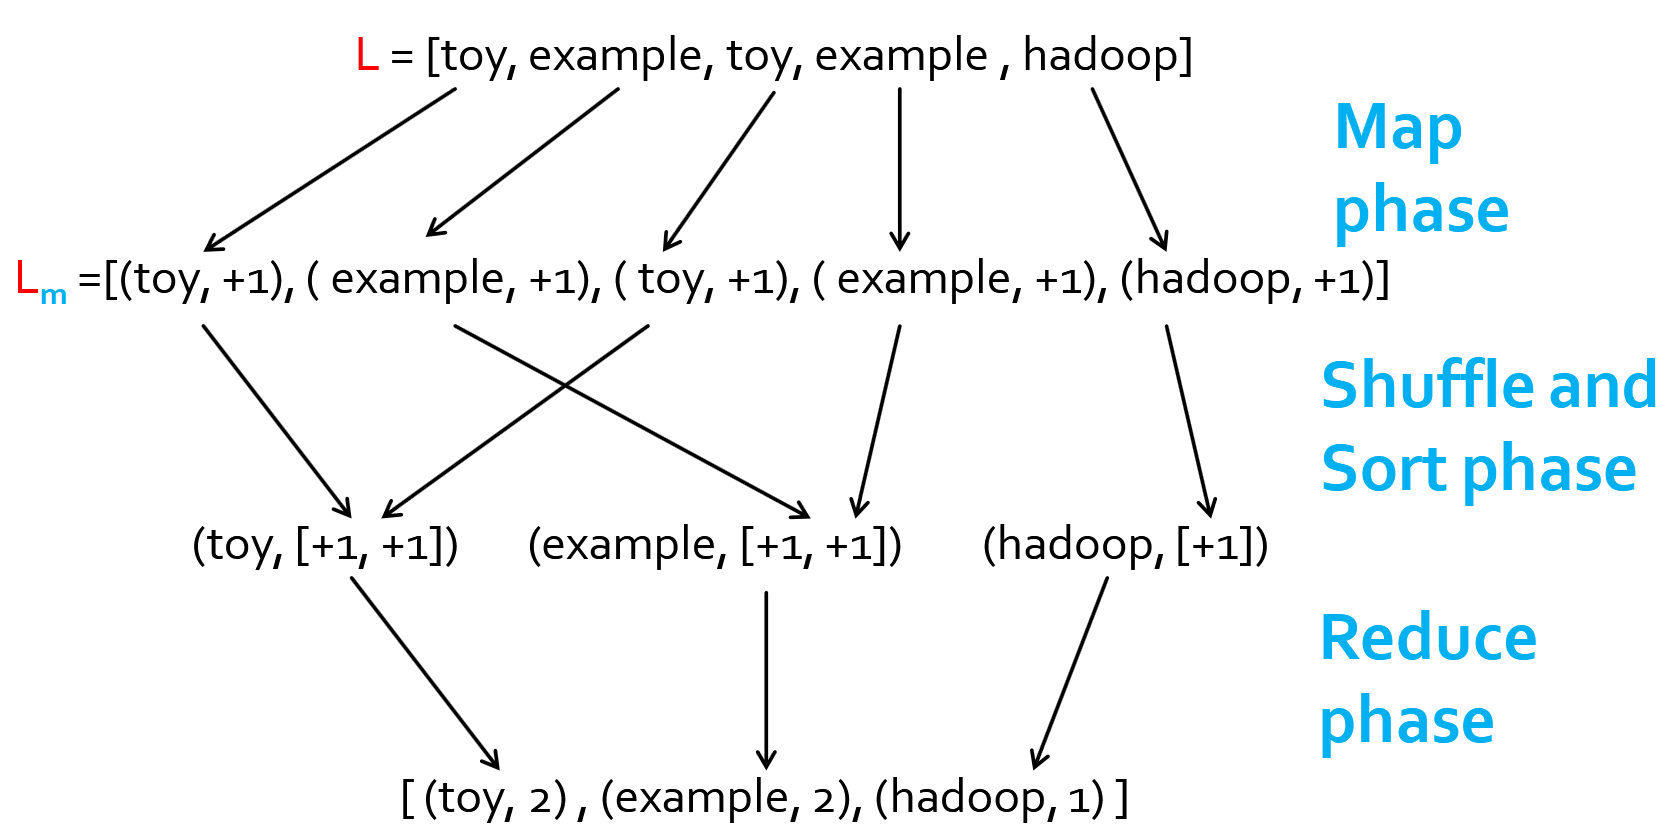
\includegraphics[width=0.8\textwidth]{capitoli/03_Intro_HadoopAndMapReduce/images/word_count_example}
    \caption{Esempio di applicazione MapReduce per il problema del Word Count.}
    \label{fig:word_count_example}
\end{figure}